\chapter{Short Rate Models}

The volume of traded interest rate derivatives in both the OTC and exchange-traded markets have been increasing sharply over the past decades. As the number of new and simultaneously exotic interest rate products virtually exploded, it has been a key challenge to find good and primarily robust procedures for pricing and also hedging these products. To reach this goal it is essential to have reliable models to describe the evolution of the interest rate with time.

In this Chapter the most common interest rate modelling techniques are reviewed together with related \texttt{python} applications.

\section{Short Rate Models}
Bond, option and other derivative prices depend only on the process followed by $r$ in a risk neutral world.
Let $Z(R, t, T)$ be the price of a zero coupon bond with maturity $T$ at time $t$. It defines the corresponding interest rate $R(T)$ by the formula

\begin{equation}
\begin{gathered}
Z(R, t, T) = e^{−R(T)(T−t)} \\
R(T) = -\cfrac{\ln Z(R, t, T)}{T − t}
\end{gathered}
\label{eq:zcb}
\end{equation}

Zero-coupon yield curve, also called term structure of interest rates, is then formed by interest rates with different maturities

The \emph{short rate} (also called \emph{instantaneous short rate}), $r(t)$, at time $t$ is the rate that applies to an infinitesimally short period at time $t$. It can be seen as the beginning of the yield curve: 

\begin{equation}
r(t) = \underset{T\rightarrow t^{+}}{lim}R(T)
\label{eq:short_rate}
\end{equation}

%The price can be expresses as
%
%\[\mathbb{E}[e^{-r(T-t)}\textrm{payoff}]\]
%
%If \(Z(t, T)\) is the price of a zero coupon bond then from the previous
%equation
%
%\[Z(t, T) = \mathbb{E}[e^{-r(T-t)}]\]

%The interest rates implied by the zero coupon bonds form a yield curve, 
%or more precisely, a zero curve.

From Equations~\ref{eq:zcb} and~\ref{eq:short_rate} it is clear that the term structure of interest rates at any time can be obtained from the value of $r$ at that time and the evolution process for $r$. They show that once the process for $r$ has been defined, everything about the initial zero curve and its evolution through time can be determined.

Short rate models have been introduced in order to be able to explore the development of the dynamics of $r(t)$. They generally owe their popularity to both their high degree of tractability and flexibility. For many models one can find explicit solutions for bond and bond option prices. They may be applied to price simple instruments in closed form or sometimes by deterministic numerical methods.

In particular, the stochastic evolution of short rate models is identified by the following generalized SDE

\begin{equation}
dr(t) = (\theta(t) − \alpha(t)r(t)) dt + \sigma(t)r(t)^{\gamma} dW
\label{eq:short_rate_sde}
\end{equation}
This equation denotes a generic Gaussian Markov process where $\theta$, $\alpha$ and $\sigma$ that in general are all deterministic functions of time and $dW$ is a Brownian motion.

\section{Equilibrium Models}\label{equilibrium-models}

Equilibrium models usually start with assumptions about how the economy works and about economic variables themselves. Then they attempt to derive a process for the short rate $r(t)$ and explore what the defined process for $r$ may imply for bond and option prices.

Thus, the key idea behind this approach is to build an economically sound model, whose output are interest rates evolved as a consequence of market equilibrium. It is important to stress that they do not automatically fit today’s term structure of interest rates, but rather the current term structure is included as an output. 

Usually the risk-neutral process for the short rate is described by a SDE analogous to Eq.~\ref{eq:short_rate_sde} where $\theta$, $\alpha$ and $\sigma$ are assumed to be function of $r$ but independent of time.

A subset of such models, called \emph{one-factor equilibrium models}, is made of those whose process for $r$ involves only one source of uncertainty (i.e. one stochastic term). 

One factor models are essentially assuming that the dynamics of the whole term structure is captured by the short rate, and its future evolution. Nevertheless, one factor models are not as restrictive as it might appear. They imply that all rates move in the same direction over any short time interval, but they do not assume that they move by the same amount. Yet, it is sometimes difficult or even infeasible to find a more or less realistic model based on one factor only.

\subsection{Vasicek Model}\label{vasicek-model}

In Vasicek model the process for $r$ is described by

\begin{equation}
dr = k(\theta - r_t)dt + \sigma dW
\label{eq:vasicek_process}
\end{equation}
where \(k\), \(\theta\) and \(\sigma\) are constants.

One important difference between interest rates and other stochastic quantities is that interest rates appear to be pulled back to some long-run average level over time. This characteristic is called \emph{mean reversion}. When $r$ is high, mean reversion tends to cause it to have a negative drift; when $r$ is low, mean reversion tends to cause it to have a positive drift.

There are real economic arguments in favor of mean reversion. When rates are high, the economy tends to slow down and there is low demand for funds from borrowers. As a result, rates decline. When rates are low, there tends to be a high demand for funds on the part of borrowers and rates tend to rise.

The Vasicek model incorporates this feature (the short rate is pulled to a level $\theta$ at a rate $k$), which is a good property, but interest rates can go negative, which instead is a very bad property.

\begin{finmarkets}
The following code implements the \texttt{VasicekModel} referring to the process described by Eq.~\ref{eq:vasicek_process}.
\end{finmarkets}

\begin{ipython}
import numpy as np

class VasicekModel:
    def __init__(self, k, theta, sigma):
        self.k = k
        self.theta = theta
        self.sigma = sigma

    def r_generator(self, r0, T, m=100):
        dt = T/m
        r = np.zeros(shape=(m,))
        r[0] = r0
        for i in range(1, m):
            r[i] = r[i-1] + self.k*(self.theta - r[i-1])*dt \   
                   + self.sigma*np.random.normal()*np.sqrt(dt)
        return r
\end{ipython}

Figure~\ref{fig:vasicek_path} shows just various realizations of the short rate using the following parameters: $r_0=0.01875$, $k=0.3$, $\theta=0.1$ and $\sigma=0.03$. 
Two facts can be noticed by this plot: each process starts at $r_0$, but is pulled towards 0.10 which is the value of $\theta$ (dashed red line), and the interest rate can drop below 0\%. The Figure also shows the expected value of the process.

\begin{figure}[htb]
    \centering
    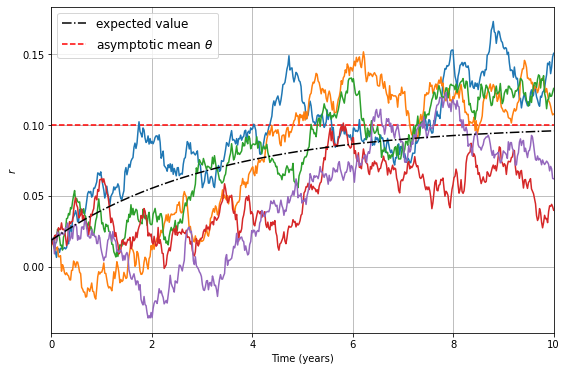
\includegraphics[width=0.7\linewidth]{figures/vasicek_short_rate}
    \caption{A realization of a path determined with Vasicek model ($k=0.3, \theta=0.1, \sigma=0.03$).}
	\label{fig:vasicek_path}
\end{figure}

\subsubsection{Vasicek Stochastic Differential Equation}
\label{vasicek-stochastic-differential-equation}

In this Section we outline the steps necessary to determine the solutions of Eq.~\ref{eq:vasicek_process}.
Multiplying both sides by \(e^{kdt}\) and rearranging the terms gives

\begin{equation*}
e^{kdt}dr_t + e^{kdt}kr_t dt = e^{kt}k\theta dt + e^{kt}\sigma dW
\end{equation*}
The left-hand side follows the product rule for the derivative

\begin{equation*}
d(e^{kdt}r_t) = e^{kdt}dr_t + e^{kdt}kr_t dt= e^{kt}k\theta dt + e^{kt}\sigma dW
\end{equation*}
Then we can integrate both sides

\begin{equation*}
\int^{t=T}_{t=s} d(e^{kdt}r_t)\,dt = \int^T_s e^{kt}k\theta dt +\int^T_s e^{kt}\sigma dW
\end{equation*}
The integral on the left-hand is trivial since \(\int^b_a\,dx = x(b)-x(a)\), so

\begin{equation*}
e^{kT}r_T - e^{ks}r_s = \int^T_s e^{kt}k\theta\,dt +\int^T_s e^{kt}\sigma\,dW
\end{equation*}
and solving for $r(T)$

\begin{equation*}
r_T=e^{-k(T-s)}r_s+ e^{-kT}\int^T_s e^{kt}k\theta\,dt +e^{-kT}\int^T_s e^{kt}\sigma dW
\end{equation*}
The second term of the right-hand side is a simple deterministic integral

\begin{equation*}
e^{-kT}\int^T_s e^{kt}k\theta\,dt=e^{-kT}k\theta\int^T_s e^{kt}d_t=e^{-kT}k\theta\frac{1}{k}(e^{kt}|^T_s)= e^{-kT}\theta(e^{kT}-e^{ks})=\theta\left(1-e^{-k(T-s)}\right)
\end{equation*}
Substituting back we get the searched solution

\begin{equation}
r_T=e^{-k(T-s)} r_s+\theta(1-e^{-k(T-s)})+ \sigma e^{-kT}\int^T_s e^{kt}\,dW
\end{equation}

The first thing to note is that the short rate is made of a deterministic term
and a stochastic integral.
Therefore, the rate is distributed like a normal Gaussian

\begin{equation*}
r_T \sim \mathcal{N}(\mathbb{E}(r_t), \textrm{var}(r_t))
\end{equation*}
We can also determine the mean and the variance of such a distribution.
Concerning the mean

\begin{equation}
\mathbb{E}(r_T)=e^{-k(T-s)} r_s+\theta\left(1-e^{-k(T-s)}\right)
\end{equation}
where the property that $\mathbb{E}(\textrm{stochastic~Integral}) = 0$ has been used.

Regarding the variance, noting that the variance of a deterministic variable is zero, we only need to calculate it for the stochastic integral. %We can do this by using the It\(\hat{o}\) Isometry,
%as the terms inside the Stochastic Integral are deterministic functions
%of time.

\begin{equation*}
\textrm{var}(r_T)=\mathbb{E}(r^2_T)-(\mathbb{E}(r_T))^2
\end{equation*}
where $(\mathbb{E}(r_T))^2 = 0$ therefore

\begin{equation}
\begin{aligned}
\textrm{var}(r_T)&=\mathbb{E}(r^2_T)=\mathbb{E}(\sigma^2 \int^T_s e^{-2k(T-t)}\,dt)=\sigma^2 e^{-2kT} \mathbb{E}( \int^T_s e^{-2k(-t)}\,dt)=\\
&=\sigma^2 e^{-2kT} \frac {1}{2k}(e^{2kT}-e^{2ks})=\sigma^2 \frac {1}{2k}(1-e^{2k(T-s)}) 
\end{aligned}
\end{equation}
where we have used that $dW^2 = dt$.
So in conclusion the distribution of the stochastic rate is

\begin{equation}
r_T \sim \mathcal{N}(e^{-k(T-s)} r_s+\theta(1-e^{-k(T-s)}),\sigma^2 \frac {1}{2k}(1-e^{2k(T-s)}))
\end{equation}

\subsubsection{Bond Pricing Equation}\label{bond-pricing-equation}

Although applied to bonds this kind of technique is more general and may be used to price many other contracts.

Since the whole idea relies on building a hedged portfolio we need to face the technical problem of the lack of an underlying asset with which
to hedge a bond (since it is a ``derivative'' of $r$). The only way to do that is by hedging one bond with another of a different maturity.

So let's set up a portfolio containing two bonds with different maturities $T_1$ and $T_2$ and price respectively $Z_1(r, t, T_1)$
and $Z_2(r, t, T_2)$. We hold one of the former and a number $\Delta$ of the latter

\begin{equation*}
\Pi = Z_1 − \Delta Z_2
\end{equation*}
The change in this portfolio in a time $dt$ is given by

\begin{equation*}
d\Pi = \cfrac{\partial Z_1}{\partial t}dt + \cfrac{\partial Z_1}{\partial r}dr + \cfrac{1}{2}\sigma^2 \cfrac{\partial^2 Z_1}{\partial r^2}dt - \Delta\left(\cfrac{\partial Z_2}{\partial t}dt + \cfrac{\partial Z_2}{\partial r}dr + \cfrac{1}{2}\sigma^2 \cfrac{\partial^2 Z_2}{\partial r^2}dt\right)
\end{equation*}
where we have applied It$\hat{o}$'s lemma to functions of $r$ and $t$. All the randomness in this expression comes from $dr$ terms given that the rate follows Eq.~\ref{eq:vasicek_process} which contains the Brownian motion $dW$. So to eliminate it (hedging) we need to choose $\Delta$ such that $dr$ terms cancelled out

\begin{equation*}
\Delta = \cfrac{\cfrac{\partial Z_1}{\partial r}}{\cfrac{\partial Z_2}{\partial r}}
\end{equation*}
So we get

\begin{equation*}
d\Pi = \cfrac{\partial Z_1}{\partial t}dt + \cfrac{1}{2}\sigma^2 \cfrac{\partial^2 Z_1}{\partial r^2}dt - \Delta\left(\cfrac{\partial Z_1}{\partial t}dt + \cfrac{1}{2}\sigma^2 \cfrac{\partial^2 Z_1}{\partial r^2}dt\right) = r\, \Pi dt = r \left(Z_1 - \Delta Z_2\right)dt
\end{equation*}
where we have used arbitrage arguments to set the return of the portfolio equal to the risk-free rate (i.e. this risk-free rate is just the spot rate). Rearranging the terms

\begin{equation*}
\cfrac{\cfrac{\partial Z_1}{\partial t} + \cfrac{1}{2}\sigma^2 \cfrac{\partial^2 Z_1}{\partial r^2} - rZ_1}{\cfrac{\partial Z_1}{\partial r}}=\cfrac{\cfrac{\partial Z_2}{\partial t} + \cfrac{1}{2}\sigma^2 \cfrac{\partial^2 Z_2}{\partial r^2} - rZ_2}{\cfrac{\partial Z_2}{\partial r}}
\end{equation*}

Since the two sides of the equation depend on $T_1$ and $T_2$ separately the only way for this to be possible is for both sides to be independent of the maturity date. So in general

\begin{equation*}
\cfrac{\cfrac{\partial Z}{\partial t} + \cfrac{1}{2}\sigma^2 \cfrac{\partial^2 Z}{\partial r^2} - rZ}{\cfrac{\partial Z}{\partial r}}= a(r, t)
\end{equation*}
for some function $a(r, t)$. A convenient definition for $a$ is $a(r, t) = \sigma(r, t )\lambda(r, t) − u(r, t)$ which leads to the bond pricing equation
\begin{equation}
\cfrac{\partial Z}{\partial t} + \cfrac{1}{2}\sigma^2 \cfrac{\partial^2 Z}{\partial r^2} + (u - \lambda\sigma)\cfrac{\partial Z}{\partial r} - rZ = 0
\label{eq:bond_pricing_equation}
\end{equation}

The function $\lambda$ is called the market price of risk since it can be interpreted as the excess return above the risk-free rate for accepting a certain level of risk.

\subsubsection{Solution for the Vasicek Model}
\label{solution-for-the-vasicek-model}
The value of a zero-coupon bond according to Eq.~\ref{eq:bond_pricing_equation} in the context of the Vasicek model is

\begin{equation} 
\begin{gathered}
Z(0, T) = e^{A(0,T)−r_0 B(0,T)} \\
B(0, T) = \cfrac{1 - e^{-kT}}{k}\\
A(0, T) = \cfrac{(B(0, T) - T)(k^2\theta - \sigma^2/2)}{k^2} - \cfrac{\sigma^2 B(0, T)^2}{4k}
\label{eq:zcb_vasicek}
\end{gathered}
\end{equation}
Furthermore
\begin{equation}
R(t, T) = \cfrac{1}{T-t} A(t,T)+\cfrac{1}{T-t}B(t, T)r(t)
\label{eq:term_structure_vasicek}
\end{equation}
showing that the entire term structure can be determined as a function of $r(t)$ once the model parameters have been chosen.

In the following code we have extended the \texttt{VasicekModel} class with new methods to compute the zero coupon bound price as described by Equations~\ref{eq:zcb_vasicek}.

\begin{ipython}
class VasicekModel:
    ...

    def _A(self, T):
        return ((self._B(T) - T)*(self.k**2*self.theta-self.sigma**2/2)/self.k**2) \
                - (self.sigma**2*self._B(T))/(4*self.k)

    def _B(self, T):
        return (1-np.exp(-self.k*T))/self.k

    def ZCB(self, T, r0):
        return np.exp(self._A(T)-r0*self._B(T))
\end{ipython}

To demonstrate some of the possible curve shapes allowed by the Vasicek model solving Eq.~\ref{eq:zcb}, Figure~\ref{fig:yield_vasicek} shows yield curves with different spot rates. Notice that the yield curve can be both increasing or decreasing with maturity.

\begin{figure}[htb]
    \centering
    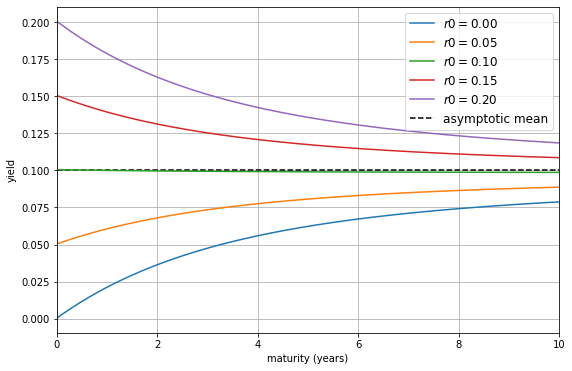
\includegraphics[width=0.7\linewidth]{figures/vasicek_yields}
    \caption{Various yield curves computed according to the Vasicek model ($k=0.5, \theta=0.1, \sigma=0.03$).}
    \label{fig:yield_vasicek}
\end{figure}

Just to cross check the bond pricing formula was implemented correctly, the price using Eq.~\ref{eq:zcb_vasicek} versus the price using Monte Carlo simulation of $\mathbb{E}\left[e^{\int_0^T r_s ds}\right]$ have been compared. The prices are in excellent agreement.

\begin{ipython}
r0 = 0.03
v = VasicekModel(0.3, 0.10, 0.03)

n = 1000
T = 1
m = 100
dt = T/m

res = []
for i in range(n):
    np.random.seed(i)
    r = v.r_generator(r0, T, m)
    I = np.sum(r[1:])*dt
    res.append(np.exp(-I))

print (f"Exact Vasicek Price: {v.ZCB(T, r0):.4f}")
print (f"MC Price: {np.mean(res):.4f}")
print (f"MC Std Error: {np.std(res)/np.sqrt(n):.4f}")
\end{ipython}
\begin{ioutput}
Exact Vasicek Price: 0.9613
MC Price: 0.9615
MC Std Error: 0.0005
\end{ioutput}

\subsubsection{Model Calibration}
In order to estimate the Vasicek model parameters from market data, it is possible to discretize the SDE of Eq.~\ref{eq:vasicek_process} as follows
\begin{equation*}
r_{t=\delta t} = r_t (1-k\delta t) + k\theta\delta t + \sigma \sqrt{\delta t}\mathcal{N}(0,1)
\end{equation*}
which can be rearranged as
\begin{equation}
r_{t+\delta t} = ar_t + b + \epsilon
\label{eq:vasicek_regression}
\end{equation}
Equation~\ref{eq:vasicek_regression} can be used in a linear regression (see Section~\ref{sec:linear-regression}) to determine the model parameters as follows
\begin{equation}
\begin{gathered}
k = \frac{1-a}{\delta t} \\
\theta = \frac{b}{1-a} \\
\sigma^2 = \frac{Var(\epsilon)}{\delta t}
\end{gathered}
\label{eq:vasicek_parameters_estimate}
\end{equation}

As an example the Vasicek model has been calibrated on the 3-months Treasury Bills monthly data since 2010 (\href{https://raw.githubusercontent.com/matteosan1/finance_course/develop/libro/input_files/TB3MS.csv}{TB3MS.csv}). Figure~\ref{fig:TB3MS} reports the scatter plot of $r(t)$ vs $r(t+1)$.

\begin{figure}[htb]
\centering
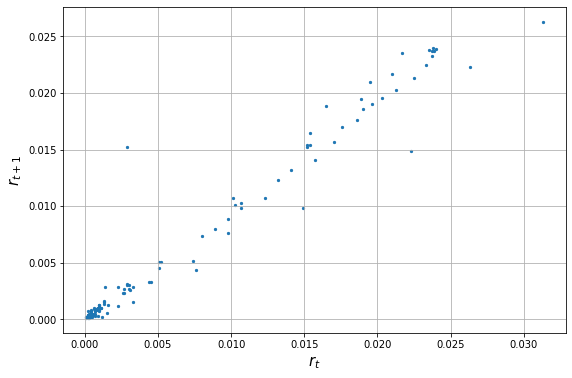
\includegraphics[width=0.7\linewidth]{figures/TB3MS}
\caption{Scatter plot of 3-months Treasury Bills data since 2010.}
\label{fig:TB3MS}
\end{figure}

The regression is performed in the following code, notice that it is necessary to remove possible \texttt{NaN} values from the dateframe for the algorithm to work. 

\begin{ipython}
import pandas as pd
import statsmodels.api as sm

df = pd.read_csv("TB3MS.csv")
df = df[df['DATE']>'2010-12-01']

df.dropna(inplace=True)
df['TB3MS'] = df['TB3MS']/100
df['prec'] = df['TB3MS'].shift(-1)

X = sm.add_constant(df['prec'][:-1])
y = df['TB3MS'][:-1]
model = sm.OLS(y, X)
r = model.fit()
print (r.summary())
\end{ipython}
\begin{ioutput}
                            OLS Regression Results                            
==============================================================================
Dep. Variable:                  TB3MS   R-squared:                       0.964
Model:                            OLS   Adj. R-squared:                  0.964
Method:                 Least Squares   F-statistic:                     3711.
Date:                Wed, 26 Oct 2022   Prob (F-statistic):          1.25e-101
Time:                        07:38:04   Log-Likelihood:                 713.32
No. Observations:                 140   AIC:                            -1423.
Df Residuals:                     138   BIC:                            -1417.
Df Model:                           1                                         
Covariance Type:            nonrobust                                         
==============================================================================
                 coef    std err          t      P>|t|      [0.025      0.975]
------------------------------------------------------------------------------
const       9.773e-05      0.000      0.625      0.533      -0.000       0.000
prec           0.9478      0.016     60.922      0.000       0.917       0.979
==============================================================================
Omnibus:                      147.784   Durbin-Watson:                   1.043
Prob(Omnibus):                  0.000   Jarque-Bera (JB):             7494.971
Skew:                           3.357   Prob(JB):                         0.00
Kurtosis:                      38.210   Cond. No.                         123.
==============================================================================
\end{ioutput}

The most interesting part of the summary is, at least for our purpose: 

\begin{itemize}
\item \texttt{R-squared}: the closer to 1 the higher is the linear correlation between $y$ and $X$;
\item coeff column: the \texttt{prec} (our $\beta$) resulting from the regression, represent the mean change in the response variable $y$ for one unit of change in the predictor variable $X$ (\texttt{const} is the corresponding $\alpha$);
\item  \texttt{P>|t|} column: the p-value for each term tests the null hypothesis that the coefficient is equal to zero (no effect). A low p-value (< 0.05) indicates that you can reject the null hypothesis. In other words, a predictor that has a low p-value is likely to be a meaningful addition to your model because changes in the predictor's value are related to changes in the response variable.
Conversely, a larger (insignificant) p-value suggests that changes in the predictor are not associated with changes in the response.
\end{itemize}

The corresponding parameter values have been estimated using Eqs.~\ref{eq:vasicek_parameters_estimate}
\begin{ipython}
import numpy as np

dt = 1/12
theta = r.params['const']/(1-r.params['prec'])
k = (1-r.params['prec'])/dt
sigma = (np.sqrt(np.var(r.resid)))/dt
print (f"k: {k:.3f}, theta: {theta:.4f}, sigma: {sigma:.3f}")
\end{ipython}
\begin{ioutput}
k: 0.627, theta: 0.0019, sigma: 0.018
\end{ioutput}
Few realizations of $r(t)$ with the calibrated model are shown in Figure~\ref{fig:vasicek_calibrated_paths}.

\begin{figure}[htb]
\centering
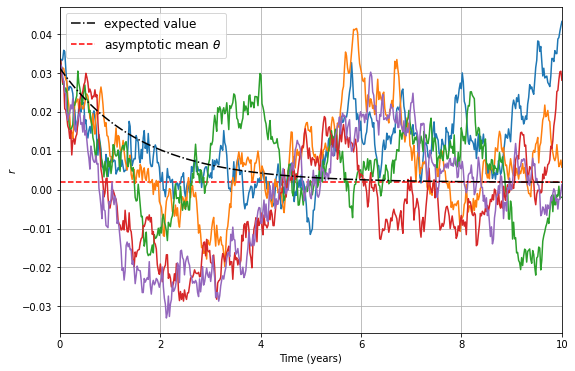
\includegraphics[width=0.7\linewidth]{figures/vasicek_calibrated_paths}
\caption{Realizations of $r(t)$ with the Vasicek calibrated model ($k=0.63, \theta=0.0019, \sigma=0.018$).}
\label{fig:vasicek_calibrated_paths}
\end{figure}

\subsection{Cox, Ingersoll and Ross (CIR) Model}
\label{cox-ingersoll-and-ross-cir-model}

In Vasicek model the short term interest rate, $r$ can become negative. In the CIR model this can never happen since the process is expressed as

\begin{equation}
dr = k(\theta - r_t)dt + \sigma\sqrt{r_t}dW
\label{eq:cir_process}
\end{equation}

This has still mean reverting drift but the standard deviation of the change in the short rate in a short period of time is proportional to $\sqrt{r}$. This means that, as the short-term interest rate increases, its standard deviation increases.

In CIR bond prices have similar general form as in Vasicek model $ZBC(0, T)=A(0, T)e^{B(0, T)r_0}$, where

\begin{equation}
B(t, T) = \cfrac{2(e^{\gamma(T-t)}-1)}{(\gamma+k)(e^{\gamma(T-t)}-1)+2\gamma}
\label{eq:cir_B_param}
\end{equation}

\begin{equation}
A(t, T) = \left[\cfrac{2\gamma e^{(k+\gamma)(T-t)/2}}{(\gamma+k)(e^{\gamma(T-t)}-1)+2\gamma}\right]^{2k\theta /\sigma^2}
\label{eq:cir_A_param}
\end{equation}
with $\gamma = \sqrt {k^2 + 2\sigma^2}$. As in the Vasicek model the value of $r(t)$ determines the term structure level at time $t$.

\begin{finmarkets}
The following code implements the \texttt{CIRModel} class which has similar methods to \texttt{VasicekModel} for computing short rate, and zero coupon bond value.
\end{finmarkets}

\begin{ipython}
import numpy as np

class CIRModel:
    def __init__(self, k, theta, sigma):
        self.k = k
        self.theta = theta
        self.sigma = sigma
        self.gamma = np.sqrt(self.k**2 + 2*self.sigma**2)

    def r_generator(self, r0, T, m=100):
        dt = T/m
        r = np.zeros(shape=(m,))
        r[0] = r0
        for i in range(1, m):
            r[i] = r[i-1] + self.k*(self.theta - r[i-1])*dt \
                   + self.sigma*np.random.normal()*np.sqrt(dt*r[i-1])
        return r

    def _B(self, T):
        c = np.exp(self.gamma*T) - 1
        return 2*c/((self.gamma + self.k)*c + 2*self.gamma)

    def _A(self, T):
        c = np.exp(self.gamma*T) - 1
        num = 2*self.gamma*np.exp((self.k+self.gamma)*T/2)
        den = (self.gamma + self.k)*c + 2*self.gamma
        return np.power(num/den, 2*self.k*self.theta/self.sigma**2)

    def ZCB(self, T, r0):
        return self._A(T)*np.exp(-r0*self._B(T))
\end{ipython}

Figures~\ref{fig:cir_path} and~\ref{fig:cir_yields} show respectively one simulation of the short rate and the interest rate resulting from the application of the CIR model. Notice how it remains always positive.

\begin{figure}[htb]
\centering
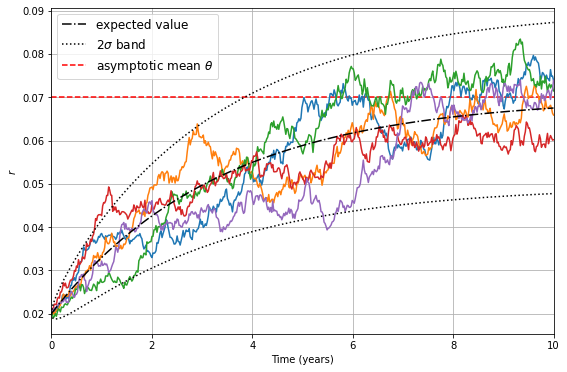
\includegraphics[width=0.7\linewidth]{figures/cir_short_rate}
\caption{Various realizations of short rate determined with CIR model ($k=0.3, \theta=0.07, \sigma=0.03$). The plot shows also the expected value and the $2\sigma$ bands.}
\label{fig:cir_path}
\end{figure}

\begin{figure}[htb]
\centering
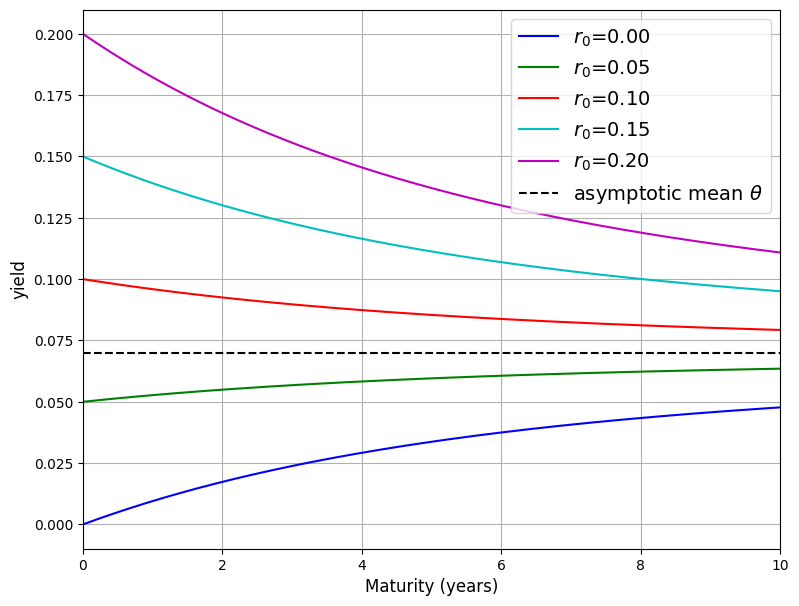
\includegraphics[width=0.7\linewidth]{figures/cir_yields}
\caption{Various yield curves computed according to the CIR model ($k=0.3, \theta=0.07, \sigma=0.03$).}
\label{fig:cir_yields}
\end{figure}

%\section{No-arbitrage Model}
%\label{no-arbitrage-model}
%
%The main disadvantage of the equilibrium, models is that they do not automatically fit today's term structure of interest rates. By choosing the appropriate parameters they can provide an approximate fit to many of the term structures but the fit is not usually exact and in some cases no reasonable fit can be found.
%
%A no-arbitrage model is designed to be exactly consistent with today's term structure of interest rates (i.e.~todas's term structure of interest rate is an input of the model). In this kind of models the drift term is in general dependent on time since the shape of the initial zero curve governs the average path taken by \(r\).
%
%However, in order to fit today’s term structure, the model parameters have to be calibrated to prevailing market data. The calibration process is responsible that a model eventually yields consistent instrument prices. Nonetheless, calibrating a model correctly is somehow burdensome and takes significant additional computing effort.
%
%%\subsection{Ho-Lee Model}\label{ho-lee-model}
%%Ho and Lee [55] did pioneer work by proposing the first no-arbitrage model consistent with the initial term structure. Allowing for time-dependent drift parameters typically makes short rate models consistent with a prevailing set of bond prices. In the continuous-time Ho-Lee model the stochastic process followed by the short rate is [55, 60, p.1020, p.184]
%%
%%This model was presented by Ho and Lee in the form of a binomial tree of
%%bond prices with two parameters: the short rate standard deviation and
%%the market price of risck of the short rate. It has since been shown
%%that the model is
%%
%%\[dr=\theta(t)dt +\sigma dW\]
%%where \(\sigma\), the instantaneous standard deviation of the short
%%rate, is constant and \(\theta(t)\) is a function of time chosen to
%%ensure that the model fits the initial term structure.
%%The variable
%%\(\theta(t)\) defines the average direction that \(r\) moves at time
%%\(t\). This is independent of the level of \(r\).
%%
%%The variable \(\theta(t)\) can be calculated analytically, it is
%%
%%\[\theta(t)=F_t(0, t) + \sigma^2 t\]
%%
%%where \(F(0, t)\) is the instantaneous forward rate for the maturity
%%\(t\) as seen at time zero and the subscript \(t\) denotes a partial
%%derivstive with respect to \(t\). As an approximantion \(\theta(t)\)
%%equals \(F_t(0, t)\). This means that the average direction that the
%%short rate will be moving in the future is approximately equal to the
%%slope of the instantaneous forward curve.
%%Similar to the Vasicek model, for every t there is a positive probability that the interest rates become negative.
%%
%%Applying Itˆo’s lemma, the SDE (6.9) can be solved explicitly for bond prices and short rates. There is an explicit formula available in the Ho-Lee model and thus the term structures are defined as
%%
%%In Ho-Lee model bond price can be determined analytically
%%
%%\[Z(t, T)=A(t, T)e^{-r(t)(T-t)}\]
%%where
%%
%%\[\ln A(t, T)=\ln\cfrac{Z(0,T)}{Z(0,t)}+(T-t)F(0,t)-\cfrac{1}{2}\sigma^2 t(T-t)^2\]
%%
%%In these equations, time zero is today, Times \(t\) and \(T\) are
%%general times in the future with \(T\geq t\). The equations, therefore,
%%define the price of a zero coupon bons at a future time \(t\) in terms
%%of the short rate at time \(t\) and the prices of bonds today. The
%%latter can be calculater from today's term structure.
%
%\subsection{Hull-White Model}
%\label{hull-white-model}
%The unsatisfactory fitting of the observed term structure of interest rates implied by the Vasicek model brought Hull and White~\cite{bib:hull_white_model} in 1990 to propose a new model that basically combines the advantages of the Vasicek and those of no-arbitrage models.
%
%As they defined it, it is an extension of the Vasicek model. However, in H-W the parameters are time dependent, what increases the possibility of calibrating them with respect to market data. The Hull-White model is growing in importance lately due to the reason that it allows the interest rates to be negative while we will not find this feature in many other models. 
%In the past, when the people surrounding the financial world thought of negative interest rates as something impossible, it was criticized for the same reason. However, nowadays reality is quite different and negative rates are all over the market. Furthermore, many specialists on the matter say they are here to stay.
%
%The explanation of why negative interest rates are possible in this model is that the short rate in Hull-White is normally distributed (it is a so-called Gaussian model), therefore:
%\begin{equation}
%dF = σ_N F dW;\quad F(0) = f
%\end{equation}
%where $σ_N$ is the normal volatility. 
%
%The Hull-White stochastic process is defined as
%\begin{equation}
%dr = \left(\theta(t) - a r \right)dt + \sigma dW
%\end{equation}
%where $a$ and $\sigma$ are constants. This can be seen as a pure no-arbitrage model with mean reversion ($a$ is the mean reverting parameter, and is defined in a way in which the drift of the process will be negative for values of $r$ greater than $\theta/a$ and vice-versa) but at the same time, as a Vasicek model with a time-dependent reversion level. Firstly, the Hull-White model makes the parameter $\theta$ time-dependent so that there are enough degrees of freedom to fit the model to the interest rate initial term structure. Here $\theta$ is a deterministic function of time and will be calibrated against the theoretical yield curve. On the other hand, $a$ and $\sigma$ should be chosen to reflect the current and future volatilities of the short-term-interest rate. So like in Vasicek model they can be fitted to the current term structure of interest rates and the current term structure of interest-rate volatility respectively.
%
%We can appreciate it better recalling the Term Structure equation with the Zero Coupon boundary condition and the Hull-White $r$-dynamics:
%\begin{equation}
%\begin{cases}
%\cfrac{\partial F^T}{\partial t} + \left[\theta(t) − a r(t)\right]\cfrac{\partial F^T}{\partial r}
%+\cfrac{1}{2}\sigma^2\cfrac{\partial^2 F^T}{\partial r^2} - r(y)F^T = 0 \\
%F(r, T, T) = 1
%\end{cases}
%\label{eq:HW_PDE}
%\end{equation}
%
%%We see that µ(t, r) − λ(t, r)σ(t) = θ(t) − a(t)r(t) and so, the drift includes the market price of risk and the volatility that should be calibrated against real data. T
%
%The analytical solution for the short rates in this model is as follows:
%\begin{equation}
%r(t) = r(s)e^{−a(t−s)} + \int_{s}^{t}e^{−a(t−u)}\theta(u)du + \sigma\int_s^t e^{−a(t−u)}dW(u)
%\end{equation}
%where
%\begin{equation}
%\theta(t) = f(0, T) + a f(0, T) + \cfrac{\sigma^2}{2a}\left(1 − e^{−aT}\right)
%\end{equation}
%and the Zero-Coupon bond price:
%\begin{equation}
%p(t, T) = A(t, T)e^{B(t,T)r(t)}
%\end{equation}
%\begin{equation}
%A(t, T) = \cfrac{p(0, T)}{p(0, t)}\textrm{exp}\left\{B(t, T)f(0, t) − \cfrac{\sigma^2}{4a}B(t, T)^2\left(1 − e^{−2at}\right)\right\}
%\end{equation}
%\begin{equation}
%B(t, T) = \cfrac{1}{a} \left(1 − e^{−a(T −t)}\right)
%\end{equation}
%with $f(0, t)$ being the forward rate and $p(0, t)$ the price of a bond starting today with maturity at time $t$.
%
%\subsection{Approximate Solution with Finite Difference}
%In this Section we are going to implement the pricing of Zero-Coupon bonds solving the Hull-White PDE through the Finite Difference Method, in particular, Crank-Nicolson~\ref{sec:finite_difference}.
%
%To solve the PDE in Eq.~\ref{eq:HW_PDE} through Crank-Nicolson we then need to define a grid with the rates as rows and time as columns. The idea behind this grid is to discretize these two variables in $N$ pieces of $h$ length equal to $d$r and $T$ pieces of $k$ length equal to $dt$. Therefore, applying the central and second central differences to both variables we get
%\begin{equation}
%\begin{cases}
%u_{i,j} = u(r_i, t_j ) \\[1ex]
%\cfrac{\partial u(r_i, t_j )}{\partial t} = \cfrac{u_{i,j+1} − u_{i,j−1}}{2k} \\[1ex]
%\cfrac{\partial u(r_i, t_j )}{\partial r} = \cfrac{u_{i+1,j} − u_{i−1,j}}{2h} \\[1ex]
%\cfrac{\partial^2 u(r_i, t_j )}{\partial r^2}=\cfrac{u_{i+1,j} + u_{i−1,j} − 2u_{i,j}}{h^2}
%\end{cases}
%\end{equation}
%Now, applying these Crank-Nicolson equalities to the Hull-White term-structure Equation~\ref{eq:HW_PDE} we have
%\begin{equation}
%\cfrac{\partial u_{i,j}}{\partial t} = r_i u_{i,j} − \left(\theta(t) − ar(t)\right) \cfrac{u_{i+1,j} − u_{i−1,j}}{2h}
%−\cfrac{1}{2}\sigma^2\cfrac{u_{i+1,j} + u_{i−1,j} − 2u_{i,j}}{h^2}
%\end{equation}
%that can be rearranged to give the multipliers of each $u_{i,j}$
%\begin{equation}
%\cfrac{\partial u_{i,j}}{\partial t} = \left(-\cfrac{\sigma^2}{2h^2}+ \cfrac{\theta(t) − a r(t))}{2h}\right)
%u_{i−1,j}+\left(\cfrac{\sigma^2}{h^2}+r_i\right)u_{i,j}−\left(\cfrac{\sigma^2}{2h^2}+ \cfrac{\theta(t) − a r(t))}{2h}\right)
%u_{i+1,j}
%\end{equation}
%Thus, letting:
%\begin{equation}
%\begin{cases}
%P_d = −\cfrac{\sigma^2}{2h^2} + \cfrac{\theta(t) − ar(t)}{2h} \\[1ex]
%P_m = \cfrac{\sigma^2}{h^2}+r_i \\[1ex]
%P_u = \cfrac{\sigma^2}{2h^2}+ \cfrac{\theta(t) − a r(t))}{2h}
%\end{cases}
%\end{equation}
%we can perform the following matrix where $t_j = jk; j = 0, 1, 2, \ldots , T$ and $r_i =ih; i = 0, 1, 2, \ldots, N$
%\begin{equation}
%A =
%\begin{bmatrix}
%P_m(r_0, t_j) & P_u(r_0, t_j) & 0 & 0 & 0 & \cdots & 0 \\
%P_d(r_1, t_j) & P_m(r_0, t_j) & P_u(r_0, t_j) & 0 & 0 & \cdots & \vdots \\
%0 & P_d(r_2, t_j) & P_m(r_2, t_j) & P_u(r_2, t_j) & 0 & \cdots & \vdots \\
%0 & 0 & P_d(r_3, t_j) & P_m(r_3, t_j) & P_u(r_3, t_j) & \cdots & \vdots \\
%\vdots & \vdots & \vdots & \vdots & \vdots & \vdots & \vdots \\
%0 & 0 & 0 & \cdots & 0 & P_d(r_N, t_j) & P_m(r_N, t_j) 
%\end{bmatrix}
%\end{equation}
%that will define the behavior of the rates every time-step $k$ passes. Letting a vector $\mathbf{u}$ represent the rates at time $j$, following Crank-Nicolson, we will have the functions that define increments in rates from $j$ to $j + 1$ as:
%\begin{equation}
%\cfrac{\mathbf{u}_{j+1} − \mathbf{u}_j}{k}=\cfrac{[A](tj)\mathbf{u}_j + [A](t_{j+1})\textbf{u}_{j+1}}{2}
%\end{equation}
%that will be solved as:
%\begin{equation}
%\textbf{u}_j = \left([I] + \cfrac{k}{2}[A](t_j)\right)^{-1}\left([I] − \cfrac{k}{2}[A](t_{j+1})\right)\mathbf{u}_{j+1}
%\end{equation}
%
%Reprocessing this calculations starting from maturity backwards for all timesteps and organizing $\mathbf{u}$ in a matrix we will get the solution for the PDE. 
%
%As we are pricing Zero-Coupon bonds, at maturity our derivatives will be worth 1. Therefore, the first boundary condition for this system of equations will be $\mathbf{u}^T = 1$ for all $i$.
%
%On the other hand, $\cfrac{\partial^2 u(r_i, t_j )}{\partial r^2}=0$ is used as boundary conditions at the first step of the grid ($P_d(r_0, t_j )$, $P_m(r_0, t_j )$ and $P_u(r_0, t_j )$).
%
%%6.3 Forward rate models
%%6 Term structure modeling
%%Forward rate models describe the arbitrage-free dynamics of the term structure of interest rates through the evolution of forward rates f (t, T ). The distinguishing feature of these models is that they explicitly describe the evolution of the full term structure, contrary to the previously discussed short rate models, which do only provide a description of the dynamics of the short rate r(t) [46, p.149]. Instantaneous short rate models, as we have seen before, are mostly easy to implement and are usually able to price many standard and also nonstandard interest rate derivatives consistently [56, p.679].
%%However, to legitimize the application of forward rate models, there are the two major limi- tations of short rate models that are generally overcome by using different types of forward rate models:
%%- In short rate models the current value of all term structure quantities is solely determined by the current value of the short rate. Thus, the term structure is entirely summarized by today’s short rate. In multifactor models the complexity of the yield curve dynamics is subsumed into the current values of a finite, but usually small number of underlying factors [46, 56, p.149, p.679f]. The new generation of correlation-dependent instruments, however, requires models that describe the state of the world by the full term structure and not necessarily by a finite number of factors, which are often not able to deal with this new dimension of complexity [92, p.311].
%%- Short rate models do not provide us with a complete freedom in the choice of the corre- sponding volatility structure. In a forward rate framework the forward rate dynamics are completely specified through their instantaneous volatility structure. In contrast, in short rate models the volatility of the short rate alone is not sufficient to fully characterize the relevant interest rate model [20, 56, 92, p.183, p.679, p.311f].
%%Forward rate models can basically be divided into two classes, namely models based on con- tinuous and simple rates, respectively. The by far most popular continuous forward rate model is the Heath, Jarrow and Morton framework. It was one of the first forward rate models pro- posed and simultaneously establishes a basis for models based on simple rates. These models are therefore closely related to the Heath, Jarrow and Morton approach and called LIBOR market models. The seemingly minor shift from continuous to simple rates has surprisingly far-reaching practical and theoretical implications [46, p.165f], as we will see later on. As in the application of both models, Heath–Jarrow–Morton as well as LIBOR market model, Monte Carlo tech- niques play a decisive role, we will give these two approaches a fundamental treatment and will implement them in Section 7 and 8, respectively.
%%52
%%
%%7 Heath, Jarrow and Morton
%%In 1992 Heath, Jarrow and Morton (hereafter, HJM) published the important paper Bond pricing and the term structure of interest rates [53] describing an alternative framework for modeling the term structure of interest rates. Under the risk-neutral measure, they derived a generalized formula for the drifts of instantaneous forward rates in terms of the volatilities of the forward rates. One of the key insights of this framework is that the HJM model is completely defined by specifying the volatilities of forward rates. Consequently, by using the observed term structure of forward rates as an input one can easily match a HJM model with the current market discount bond prices [6, p.310]
%%Basically, there are two common formulations of the model. Firstly, the price based and secondly the forward based approach. The former technique is based on the dynamics of discount bonds, i.e. it takes them as the fundamental building block. The latter directly obtains the no- arbitrage SDE which is obeyed by the forward rates [92, p.314]. For a rigorous proof of the equivalence of these two approaches it is referred to the paper of Carverhill [27]. Note, though, that, historically, the pioneering results of the HJM were first achieved in the forward rates context.
%%The virtue of the HJM theory lies in the fact that within such a framework virtually any (exogenous term structure) interest rate model can be derived. Even market models (see Section 8), for instance, have evolved starting from the instantaneous forward rate dynamics of the HJM approach. However, the disadvantage is that there are only a few volatility structures which lead to a corresponding short rate process which is indeed Markovian. This means that models of this form will, except for some wise choices of volatility specifications, which we will look at in Section 7.2, generally be path-dependent and thus non-Markovian processes [6, 20, p.310, p.184]. A short rate process can be characterized as being Markovian if its future evolution is in no way affected, in a stochastic sense, by its past realizations. If a process is indeed not influenced by its past, then the short rate process is, to use Carverhill’s [26] apt oxymoron, randomly determined [92, p.347f].
%%In general, prices of fixed-income instruments, e.g. bonds, do not depend on the values of a few individual factors but rather on the entire history of the forward rate process. This fact makes computation exceptionally difficult and often only possible by simulation since the nodes of non-recombining, or bushy trees grow exponentially and therefore the approximating lattice will literally explode already after a small number of steps [6, p.310]. As a result, Monte Carlo simulation is the computational tool of choice in the HJM setting.
%%7.1 Framework
%%As mentioned before, the HJM characterizes the dynamics of the entire forward rate curve f (t, T ), whereas 0 ≤ t ≤ T ≤ τ . The origin of any consistent implementation of the HJM approach is the current yield curve, which is obviously based on market data. This yield curve can be described either by the collection of discount bonds P(0,T) or by the instantaneous
%%forward rates f (t, T ). The forward rate at time t for date T > t is defined by [46, 53, 92, p.150, p.79, p.314]
%%∂lnP(t,T) ∂T
%%By solving the differential equation of Expression (7.1) the relationship between forward rates, spot rates and bond prices become obvious. In particular, spot rates, r(t,T), and bond prices, P(t,T), are written in terms of forward rates, f(t,T), as
%%and
%%r(t, T ) = P(t,T) = exp −
%%f(t,T) = −
%%. (7.1)
%%1T T−tt
%%f (t, s)ds 
%%f(t,s)ds ,
%%
%%respectively, for all T ∈ [0,τ], t ∈ [0,T] [6, 53, 92, p.310, p.80, p.314]. Note that the spot rate at time t, r(t), is exactly the same as the instantaneous forward rate at time t for date t, i.e., r(t) = f (t, t) [53, p.80].
%%In the HJM setting, the dynamics of the instantaneous forward rate curve are specified, under a given measure, through the SDE [46, 53, 60, p.150, p.80f, p.200]
%%df(t,T) = α(t,T,ω)dt+σ(t,T,ω)dW(t), (7.4)
%%where ω is a vector containing the past and present values of interest rates as well as bond prices at time t in the sample space Ω. The process W is a standard d-dimensional Brownian motion, whereas d is the number of factors or volatility curves which describe the forward rates. Thus, the HJM approach can be constructed as a one factor as well as a multifactor model.
%%Due to the absence of arbitrage, requested by the no-arbitrage condition, asset prices must
%%be martingales when divided by the numeraire, which in this case is exp 0t r(s)ds. However,
%%forward rates and asset prices are by no means the same. Therefore, the restrictions imposed
%%on the dynamics in (7.4) with the purpose to avoid any arbitrage opportunities are different.
%%Nevertheless, asset prices, particularly bonds, serve as a starting point in order to find theset
%%restrictions. To ensure that the discounted bond prices P (t, T ) exp − r(s)ds are positive
%%0
%%martingales, Heath et al. [53, p.81f] derived the dynamics of the form dP(t,T)
%%P(t,T) =r(t)dt+v(t,T,ω)dW(t), (7.5)
%%where 0 ≤ t ≤ T ≤ τ [46, 60, p.151, p.200]. The volatilities of the bonds v(t, T, ω) may either be functions of observed bond prices or, equivalently, of current forward rates since (7.1) indicates that they are one-to-one related to each other. Applying Itˆo’s formula yet again, Heath et al. showed [53, p.80ff] that forward rate volatilities may be derived from bond price volatilities and we therefore must have
%%∂ ∂T
%%σ(t,T,ω) = − 54
%%v(t,T,ω)
%%and T
%%v(t, T, ω) = − σ(t, s)ds + constant, (7.6)
%%t
%%simultaneously [46, p.152]. Notice, however, that P (t, T ) approaches 1 as t → T and therefore we must have v(T,T,ω) = 0 because bond’s price volatility declines to zero at maturity [92, p.318]. Thus the constant in Equation (7.6) is zero which allows us to rewrite the expression for α as [20, 46, 60, p.186, p.152f, p.200f]
%%
%%α(t, T, ω) = σ(t, T, ω) σ(t, s)ds = σi(t, T, ω) σi(t, s)ds. (7.7)
%%t i=1 t
%%This expression represents the risk-neutral drift imposed by the no-arbitage condition. Addition- ally, (7.7) reveals a key result of the HJM research activities. The assumption of arbitrage-free dynamics has led to a specific relationship between the drift and the volatility. Namely that the drift of the dynamics in (7.4) is completely determined by the volatility structure of the instantaneous forward rates. Thus we know that the HJM drifts themselves are simply a function of the volatilities, either of forward rates, or of discount bonds. If we substitute (7.7) into (7.4) then the new HJM dynamics are [46, 53, 92, p.152, p.89f, p.318ff]
%%
%%df(t,T)= σ(t,T,ω) σ(t,s)ds dt+σ(t,T,ω)dW(t). (7.8)
%%t
%%This SDE defines the no-arbitrage dynamics of the forward rate curve under the risk-neutral measure and is simultaneously the central insight of the HJM approach. Recall why the model eventually fulfills the required no-arbitrage condition. While deriving the forward rate restriction (7.7) and the corresponding dynamics (7.8), a proper specification of the drift was chosen in order to guarantee the absence of arbitrage, or more precisely, to make the discounted bond prices martingales. However, integrating (7.8) leads to the dynamics of f(t,T
%%f(t,T) = f(0,T)+ σ(u,T,ω) σ(u,s)dsdu+ σ(s,T,ω)dW(s), (7.9)
%%0u0
%%which are completely determined once the vector volatility function σ is specified [20, 53, p.186, p.89f]. Only a small step takes us now from the dynamics of the forward rates to the dynamics of the zero coupon bond price P(t,T):
%%dP(t,T)=P(t,T) r(t)dt− σ(t,s)ds dW(t) , (7.10)
%%t
%%where r(t) denotes the instantaneous short term interest rate at time t. The dynamics of r(t) are given by [20, 53, p.186, p.90]
%%
%%r(t) = f (t, t) = f (0, t) + σ(u, t, ω) σ(u, s)ds du + σ(s, t, ω)dW (s). (7.11)
%%0u0
%
%%The decisive discrepancy between HJM and previously discussed instantaneous short rate models has become apparent. We know that the HJM drift is determined once the volatility is finally specified. In contrast, the derivation of the short rate models disclosed that their dynamics and thus their drift parameters could be completely specified independent of any diffusion coefficients. Even though no volatility structures were taken into account, there was still no arbitrage introduced. A wise choice of the drift parameters is indeed crucial for calibrating short rate models to the observed bond prices. Provided that the initial forward rate curve is chosen in a way that the consistency, implied by (7.1), is guaranteed, the HJM model, however, is automatically calibrated to prevailing bond prices. To conclude, while calibrating a HJM model the initial forward curve conditions rather than individual parameters are essential. With regard to the calibrating process of a HJM framework itself, the main effort lies in choosing σ properly to firstly match bond prices and eventually the market prices of interest rate derivatives [46, 60, 92, p.153, p.200, p.312f].
%%7.2 Volatility functions
%%The proceeding section has already foreshadowed that the consequences of the choice of volatility specification for the implementation and simulation of a HJM model are enormous. The short rate process (7.11) is, as mentioned before, not a Markov process in general. However, there are suitable specifications of the volatility function σ(t, T, ω) for which r(t) is yet Markovian [20, 60, p.186f, p.203f]. For an extensive treatment of Markovian short rate processes it is referred to either the paper of Carverhill [26] or the Chapter 16 of Rebonato [92, p.347-359]. In the general case when σ(t,T,ω) is not Markovian, we may encounter major computational problems when discretizing the Dynamics (7.11) for the pricing of even simple derivatives. However, several standard Markovian functional forms for σ(t,T,ω) have been explored. Two of them, both single factor models (d = 1), are listed and shortly explained below [60, p.203]:
%%- Constant σ: σ(t, T, ω) ≡ σ.
%%In this one factor model with constant volatility each increment dW(t) moves the entire forward curve, i.e. all existing points on the curve, by an equal amount of σdW(t). Thus, the forward curve is constrained to move only in parallel [46, p.153]. For this particularly simple specification, bond prices are assumed to be lognormal and all forward rates are normal and exhibit exactly the same volatility. If these distributional assumptions are fulfilled, the according models are qualified as Gaussian [92, p.317f]. They are analytically well-tractable but also unrealistic to some extent, what we will see later on. If we insert σ into Equation (7.7) the resulting drift of a HJM model with constant σ has the form [46, p.153]
%%T
%%α(t, T, ω) = σ σ ds = σ2(T − t).
%%t
%%Solving (7.8) with constant σ leads to the dynamics of the forward rates f(t,T)=f(0,T)+ 12σ2[T2 −(T −t)2]+σW(t),
%%which is simultaneously the continuous-time equivalent of the Ho-Lee model [60, 92, p.202, p.318].
%%Flesaker [40] conducted an empirical test about the constant volatility version of the HJM model for Eurodollar futures and futures options. He found that this general version of the HJM model is unable to explain cross-sectional pricing pattern of futures options and that it exhibits systematic biases, why the model is eventually soundly rejected. Moreover, he observed that the model tends to overvalue short-term options relative to long-term options. Accordingly, he clearly motivated further empirical studies of HJM models where the volatility is allowed to vary over time rather than artificially kept constant.
%%-Exponentialσ: σ(t,T,ω)=σexp(−λ(T−t)),forsomeconstantsσ,λ>0.
%%This diffusion term σ(t,T,ω) has a greater impact on forward rates for short maturities than on forward rates for long maturities [46, p.154]. Due to this fact the HJM model in- cluding an exponential σ is eventually completely equal to the general short rate dynamics proposed by Hull and White [57], see (6.11). This makes clear that one can establish a one-to-one equivalence between the HJM one factor model and the general formulation of the Gaussian one factor instantaneous short rate model of Hull and White [20, p.187].
%%This volatility specification keeps its analytical tractability but is able to perform slightly better than the HJM model with constant σ. Yet, the results are still unsatisfactory and therefore the HJM model including exponential volatility is also rejected [60, p.203].
%%Asides from many standard approaches with the goal of finding suitable specifications of σ(t,T,ω), which make the short rate process indeed Markovian, there have been developed some more sophisticated techniques, too. They basically exploit that, even though a short rate process might not be Markovian, there may yet exist a higher-dimensional Markov process that possesses the instantaneous short rate as one of its components [20, p.188]. Ritchken and Sankarasubramanian [95], for instance, proposed a model for simply capturing the path dependence of the short rate r(t) through a single statistic. In particular, they found a few necessary and sufficient conditions which are imposed on the volatility structure of the forward rates. These conditions enable them to control the short rate’s path dependence and make them analytically tractable [20, 60, p.189, p.205].
%%A second model, which was proposed by Mercurio and Moraleda [78], derives an interest rate model within the HJM framework which explicitly assumes a humped volatility structure in the instantaneous forward rate dynamics and thus is also analytically tractable. They motivate their assumption of a humped volatility structure by the fact that forward rates themselves commonly exhibit humped volatility functions that are generally implied by simple market quotes. They have shown that their model consequently outperforms similar existing models, which do not explicitly contain such a humped shape in volatilities [20, 78, p.191f, p.213].
%%      
    
\section*{Exercises}
\begin{question}
Assume that company A has agreed to pay a 6-month Libor and receive a fixed interest rate of 8\% per year (with interest payable every six months) from the face value of \$100 million. Swap is 1.25 years to expire. The interest rates for 3, 9 and 15 months are: 10\%, 10.5\% and 11\% respectively. Assume that interest rates are continously compounded. The 6-month Libor is currently 10.2\%. 

Calculate the value of this swap for company A.
\end{question}


%  Add to \texttt{finmarkets} module a class to valuate swaptions, it should have as attributes the underlying IRS, the swap rate volatility and the question date.
%  The class should have the capability of estimating the payoff of the swaptions both with the Black-Scholes formula and Monte Carlo Simulation.
%\end{question}
%
%\begin{solution}
%	class InterestRateSwaption:
%	def __init__(self, exercise_date, irs):
%	self.exercise_date = exercise_date
%	self.irs = irs
%	def npv_bs(self, discount_curve, libor_curve, sigma):
%	A = self.irs.annuity(discount_curve)
%	S = self.irs.swap_rate(discount_curve, libor_curve)
%	T = (self.exercise_date - discount_curve.today).days / 365
%	d1 = (math.log(S/self.irs.fixed_rate) + 0.5 * sigma**2 * T)
%	/ (sigma * T**0.5)
%	d2 = d1 - (sigma * T**0.5)
%	npv = self.irs.notional * A * (S * scipy.stats.norm.cdf(d1) -
%	self.irs.fixed_rate * scipy.stats.norm.cdf(d2))
%	return npv
%	
%	def npv_mc(self, discount_curve, libor_curve, sigma, n_scenarios=10000):
%	A = self.irs.annuity(discount_curve)
%	S = self.irs.swap_rate(discount_curve, libor_curve)
%	T = (self.exercise_date - discount_curve.today).days / 365
%	discounted_payoffs = []
%	for i_scenario in range(n_scenarios):
%	S_simulated = S * math.exp(-0.5 * sigma * sigma * T +
%	sigma * math.sqrt(T) * numpy.random.normal())
%	
%	swap_npv = self.irs.notional * (S_simulated - self.irs.fixed_rate) * A
%	discounted_payoffs.append(max(0, swap_npv))
%	npv_mc = numpy.mean(discounted_payoffs)
%	npv_error = 3 * numpy.std(discounted_payoffs) / math.sqrt(n_scenarios)
%	return npv_mc, npv_error
%\end{ipython}

\begin{question}
Suppouse that the LIBOR Forward rates and the discount curve are those defined in
\href{https://github.com/matteosan1/finance_course/raw/develop/libro/input_files/libor_curve.xlsx}{libor\_curve.xlsx} and \href{https://github.com/matteosan1/finance_course/raw/develop/libro/input_files/discount_curve.xlsx}{discount\_curve.xlsx} respectively.
Determine the value of an option to pay a fixed rate of 4\% and receives LIBOR on a 5 year swap starting in 1 year. Assume the notional is 100 EUR, the exercise date is on October, 30th 2020 and the swap rate volatility is 15\%.

\noindent\textbf{Hint:} add \texttt{InterestRateSwap} class to \texttt{finmarkets.py}.
\end{question}

\cprotEnv\begin{solution}
\begin{ipython}
from finmarkets import InterestRateSwap
from datetime import date
from dateutil.relativedelta import relativedelta
from curve_data import discount_curve, libor_curve
from scipy.stats import norm
import math

pricing_date = date.today()
start_date = date.today() + relativedelta(years=1)
exercise_date = date(2020, 10, 30)

irs = InterestRateSwap(start_date, 100, 0.04, 12, 5)
sigma = 0.15
A = irs.annuity(discount_curve, pricing_date)
S = irs.swap_rate(discount_curve, libor_curve, pricing_date)
T = (exercise_date - pricing_date).days / 365
d1 = (math.log(S/irs.fixed_rate) + 0.5 * sigma**2 * T) / (sigma * T**0.5)
d2 = (math.log(S/irs.fixed_rate) - 0.5 * sigma**2 * T) / (sigma * T**0.5)
npv = irs.notional * A * (S * norm.cdf(d1) - irs.fixed_rate * norm.cdf(d2))

print("Swaption NPV: {:.3f} EUR".format(npv))
\end{ipython}
\begin{ioutput}
Swaption NPV: 13.587 EUR
\end{ioutput}
\end{solution}


\begin{thebibliography}{9}
\bibitem{bib:vasicek}O.A. Vasicek \emph{An Equilibrium Characterization of the Term Structure},
Journal of Financial Economics, 5 (1977); 177-188
\bibitem{bib:lee}T.S.Y. Ho and S.B. Lee, \emph{Term Structure Movements and Pricing Interest
Rate Contingent Claims}, Journal of Finance, 41 (December 1986): 1011-29
\bibitem{bib:irs security}J. Hull and A. White, \emph{Pricing Interest Rate Derivative Securities}, Review of Financial Studies, 3, 4 (1990): 573-92.
\end{thebibliography}

    
